\documentclass[12pt, letterpaper]{article}

% ==========================================
%              DOCUMENT PACKAGES
% ==========================================

% --- Core Language & Encoding ---
\usepackage[english]{babel} % Sets the language and regional settings for English documents
\usepackage[utf8]{inputenc} % Allows the use of UTF-8 characters in the document
\usepackage[T1]{fontenc} % Specifies the font encoding
\usepackage[margin=1.5cm]{geometry} % Sets the page margins

% --- Colors & Graphics ---
\usepackage[table,dvipsnames]{xcolor} % Advanced color management
% \usepackage{color} % Basic package for text and background colors
\usepackage{graphicx} % Enhanced support for including external images and scaling them
\usepackage{adjustbox} % Adjusts the size, scaling, and alignment of boxes, images, and tables
% \usepackage{background} % Allows adding background images or watermarks to pages
\usepackage{float} % Improves the interface for floating objects and adds the [H] placement
\usepackage{pdflscape} % Makes landscape pages display correctly on screen in PDF viewers
\usepackage{pdfpages} % Allows the inclusion of external multi-page PDF documents

% --- Math, Science & Engineering ---
\usepackage{amsfonts} % Provides extended mathematical fonts
\usepackage{amsmath} % Provides advanced mathematical typesetting and environments
\usepackage{amssymb} % Provides extended mathematical symbols
% \usepackage{amsmath, amssymb} % (Redundant combination line omitted for stability)
\usepackage{amsthm} % Facilitates the creation of theorem-like environments
\usepackage{mathtools} % Enhances amsmath with additional math tools and bug fixes
\usepackage{thmtools} % Extensions and customization options for theorem environments
\usepackage{nicematrix} % Enhances matrices and tabulars using PGF/TikZ
\usepackage{xy} % Typesets complex graphs and diagrams
\usepackage{circuitikz} % Allows drawing of electrical networks and circuits

% --- Typography & Fonts ---
\usepackage{avant} % Sets the default sans-serif font to Avant Garde
\usepackage{cantarell} % Sets the default sans-serif font to Cantarell
\usepackage{charter} % Sets the default roman font to Charter
\usepackage{cmbright} % Sets the font family to Computer Modern Bright 
\usepackage{helvet} % Sets the default sans-serif font to Helvetica
\usepackage{inconsolata} % Sets the default typewriter (monospace) font to Inconsolata
\usepackage{iwona} % Sets the font family to Iwona 
\usepackage{kurier} % Sets the font family to Kurier 
\usepackage{lmodern} % Loads the Latin Modern fonts 
\usepackage{textcomp} % Provides additional text symbols
\usepackage{ulem} % Provides various types of text underlining and strikethroughs

% --- Tables & Lists ---
\usepackage{array} % Extends the array and tabular environments
\usepackage{arydshln} % Allows dashed lines in arrays and tables
\usepackage{bigstrut} % Adds custom vertical space in table rows
\usepackage{booktabs} % Enhances the quality of tables with better horizontal rules
% \usepackage{colortbl} % Allows coloring of rows, columns, and individual cells in tables
\usepackage{diagbox} % Creates table cells with diagonal lines 
\usepackage{enumitem} % Provides advanced control over list environments
\usepackage{longtable} % Allows tables to break across multiple pages
\usepackage{multirow} % Allows individual table cells to span across multiple rows
\usepackage{tabularx} % Creates tables with dynamically adjustable-width columns
\usepackage{pgfplotstable} % Reads and cleanly formats numerical tables directly from CSV

% --- Formatting, Layout & UI ---
\usepackage{blindtext} % Generates dummy text for testing document layouts
\usepackage{caption} % Customizes captions in floating environments
\usepackage{comment} % Allows you to block out large sections of text
\usepackage{emptypage} % Automatically removes headers and footers on empty pages
\usepackage{fancyhdr} % Allows complete customization of headers and footers
\usepackage{fancyvrb} % Enhanced verbatim environments for writing raw code
\usepackage{framed} % Creates framed, shaded, or differently highlighted text regions
\usepackage{fullpage} % Quickly sets all page margins to 1 inch
\usepackage{lipsum} % Generates Lorem Ipsum dummy text
\usepackage{mdframed} % Creates highly customizable framed environments
\usepackage{multicol} % Allows intermixing single and multiple text columns
\usepackage{parskip} % Replaces standard paragraph indentation with vertical spacing
\usepackage{setspace} % Controls line spacing (single, one-and-a-half, double)
\usepackage{subcaption} % Supports sub-figures and sub-tables with independent captions
% \usepackage{subfig} % Older package for sub-figures (subcaption is generally preferred now)
\usepackage{tcolorbox} % Creates heavily customized colored and framed text boxes
\usepackage{titlesec} % Customizes the formatting of section, subsection, and chapter headings
\usepackage{titling} % Provides advanced control over the typesetting of the document title

% --- Bibliographies & References ---
\usepackage{biblatex} % Advanced, modern bibliographic processing and formatting
\usepackage{csquotes} % Context-sensitive quotation facilities
\usepackage{makeidx} % Supports the generation of a document index
% \usepackage{natbib} % Flexible bibliography support, particularly for author-year citation styles

% --- TikZ & Plotting ---
\usepackage{tikz} % Advanced package for creating vector graphics and diagrams programmatically
\usepackage{pgf-pie} % Draws pie charts programmatically using PGF/TikZ
\usepackage{pgfplots} % Creates high-quality mathematical plots, charts, and graphs
% \usepackage{fancytikzposter} % Used to create large format academic posters using TikZ

% --- URLs & Hyperlinks ---
\usepackage{url} % Formats and properly hyphenates long URLs
\usepackage{breakurl} % Allows line breaks in URLs, especially when compiled with latex -> dvips
\usepackage{hyperref} % Creates cross-referencing, clickable links, and PDF bookmarks

% --- Code Formatting ---
\usepackage{listings} % Typesets programming source code with formatting and syntax highlighting


% ==========================================
%           DOCUMENT CONFIGURATION
% ==========================================

% Custom color definitions
\definecolor{mygray}{gray}{0.9}

% Hyperlink configuration
\hypersetup{
    colorlinks=true,
    linkcolor=blue,
    urlcolor=blue
}

% Configuración adicional para breaks en URLs
\def\UrlBreaks{\do\/\do-\do_\do.\do=\do?\do\&}
\expandafter\def\expandafter\UrlBreaks\expandafter{\UrlBreaks\do\a\do\b\do\c\do\d\do\e\do\f\do\g\do\h\do\i\do\j\do\k\do\l\do\m\do\n\do\o\do\p\do\q\do\r\do\s\do\t\do\u\do\v\do\w\do\x\do\y\do\z}
\newcommand{\code}[1]{\path{#1}}

%Uncomment the following lines to use a sans-serif font
\renewcommand{\familydefault}{\sfdefault}

% TikZ libraries
\usetikzlibrary{arrows.meta, backgrounds, fit, shapes.geometric, positioning, decorations.pathreplacing}

\graphicspath{ {./img/} } % Sets the path for the graphics

\newlist{biblio}{enumerate}{1}
\setlist[biblio,1]{label=[\arabic*]}

\makeindex

% \tiny
% \scriptsize
% \footnotesize
% \small
% \normalsize (default size)
% \large
% \Large
% \LARGE
% \huge
% \Huge

% ==========================================
%         GLOBAL LISTINGS SETTINGS
% ==========================================
\lstset{
	basicstyle=\ttfamily\small,
	numbers=left,
	numberstyle=\tiny\color{gray},
	stepnumber=1,
	numbersep=10pt,
	backgroundcolor=\color{white},
	showspaces=false,
	showstringspaces=false,
	breaklines=true,
	frame=single,
	tabsize=2, 
    captionpos=b, 
    lineskip=-1pt,
	extendedchars=true,
	literate={á}{{\'a}}1 {é}{{\'e}}1 {í}{{\'i}}1 {ó}{{\'o}}1 {ú}{{\'u}}1 {Á}{{\'A}}1 {É}{{\'E}}1 {Í}{{\'I}}1 {Ó}{{\'O}}1 {Ú}{{\'U}}1 {ñ}{{\~n}}1 {Ñ}{{\~N}}1 {¿}{{\textquestiondown}}1 {¡}{{\textexclamdown}}1
}

% ==========================================
%            LANGUAGE: SQL
% ==========================================
\lstdefinestyle{sqlstyle}{
	language=SQL,
	keywordstyle=\color{blue}\bfseries,
	commentstyle=\color[rgb]{0,0.5,0}\itshape,
	stringstyle=\color{red}
}

% ==========================================
%            LANGUAGE: VHDL
% ==========================================
\lstdefinelanguage{VHDL}{
	morekeywords={entity, architecture, signal, port, in, out, inout, begin, end, process, if, then, else, elsif, case, when, others, for, while, loop, wait, library, use, std_logic, std_logic_vector, integer, boolean, rising_edge, falling_edge, component, generic, map, downto, to, and, or, not, xor, nand, nor, xnor},
	morecomment=[l]{--},
	morestring=[b]",
	sensitive=false,
	alsoletter={_}
}

\lstdefinestyle{vhdl}{
	language=VHDL,
	keywordstyle=\color{blue}\bfseries,
	commentstyle=\color[rgb]{0,0.6,0}\itshape,
	stringstyle=\color{red}
}

% ==========================================
%              LANGUAGE: C
% ==========================================
\lstdefinestyle{cstyle}{
	language=C,
	keywordstyle=\color{blue}\bfseries,
	commentstyle=\color[rgb]{0,0.5,0}\itshape,
	stringstyle=\color{red},
	directivestyle=\color{purple},
    tabsize=4 % Overrides the global tabsize of 2 for C code specifically
}

% ==========================================
%             LANGUAGE: C++
% ==========================================
\lstdefinestyle{cppstyle}{
	language=C++,
	keywordstyle=\color{blue}\bfseries,
	commentstyle=\color[rgb]{0,0.5,0}\itshape,
	stringstyle=\color{red},
	directivestyle=\color{purple},
    tabsize=4
}

% ==========================================
%           LANGUAGE: PYTHON
% ==========================================
\lstdefinestyle{pythonstyle}{
	language=Python,
	keywordstyle=\color{blue}\bfseries,
	commentstyle=\color[rgb]{0,0.5,0}\itshape,
	stringstyle=\color{red},
    % Python relies heavily on indentation, so keeping tabsize aligned is important
    tabsize=4
}

% ==========================================
%             LANGUAGE: BASH
% ==========================================
\lstdefinestyle{bashstyle}{
	language=bash,
	keywordstyle=\color{blue}\bfseries,
	commentstyle=\color[rgb]{0,0.5,0}\itshape,
	stringstyle=\color{red},
    % Bash variables often use $, so we can highlight them dynamically if needed
    moredelim=[s][\color{orange}]{\$\{}{\}}
}

% ==========================================
%           LANGUAGE: ASSEMBLY
% ==========================================
\lstdefinestyle{asmstyle}{
	language=[x86masm]Assembler,
	keywordstyle=\color{blue}\bfseries,
	commentstyle=\color[rgb]{0,0.5,0}\itshape,
	stringstyle=\color{red},
    % Adding common ARM/Microcontroller instructions for better highlighting
    morekeywords={ldr, str, mov, cmp, add, sub, b, bl, bx, push, pop, svc, eor, and, orr, lsl, lsr}
}
% % Configure header
\setlength{\headheight}{28pt} % Adjust header height for two-line header
\pagestyle{fancy}
\fancyhf{} % Clear all header and footer fields
\lhead{\textbf{Nombre:} Ugartechea González Luis Antonio -- 320223822 \\ \textbf{Asignatura:} <asignatura>, \textbf{Grupo:} <grupo>}
\renewcommand{\headrulewidth}{0.4pt}

\begin{document}

\newgeometry{margin=1.5cm}
\begin{titlepage}
    \noindent
    \renewcommand{\arraystretch}{1.5}
    % Definimos la tabla principal con dos columnas exactamente iguales (50/50)
    \begin{tabularx}{\textwidth}{|>{\centering\arraybackslash}X|>{\centering\arraybackslash}X|}
        \hline
        % Fila superior: Combinamos las dos columnas e insertamos una sub-tabla
        \multicolumn{2}{|@{}c@{}|}{%
            \begin{tabularx}{\dimexpr\textwidth-2\arrayrulewidth\relax}{m{3.5cm}|>{\centering\arraybackslash}X}
                \centering \vspace{0.2cm} 
\includegraphics[width=2cm,height=2.5cm]{escudoFI_color.png} & \large \textbf{Fundamentos de Sistemas Embebidos}
            \end{tabularx}%
        } \\
        \hline
        % Fila inferior: Alineada a la mitad exacta
        \large Facultad de Ingeniería & \large UNAM \\
        \hline
    \end{tabularx}

    \vspace{0.5cm}

    \begin{center}
        {\fontsize{35}{48}\selectfont Laboratorio de Fundamentos de} \\
        {\fontsize{35}{48}\selectfont Sistemas Embebidos\par}
        % Línea divisoria azul (se puede ajustar el tono de azul)
        \textcolor{MidnightBlue!70}{\rule{\textwidth}{1pt}}
    \end{center}

    \vspace{2cm}

    \begin{center}
        % Aumenta el espaciado entre filas para que coincida con el formato
        % \renewcommand{\arraystretch}{1.8}
        \fontsize{15}{21}\selectfont
        % Columna 1: Alineada a la derecha, en cursiva (itshape) y de 4.5cm de ancho
        % Columna 2: Alineada a la izquierda
        \begin{tabular}{>{\raggedleft\arraybackslash\itshape}p{4.5cm} @{\hspace{0.5cm}} l}
            Profesor(a): & \underline{\makebox[10cm][l]{ Eduardo Fragoso Navarro}} \\
            Asignatura: & \underline{\makebox[10cm][l]{ Fundamentos de Sistemas Embebidos}} \\
            Grupo: & \underline{\makebox[10cm][l]{3}} \\
            No de Práctica(s): & \underline{\makebox[10cm][l]{}} \\
            Integrante(s): & \underline{\makebox[10cm][l]{Tepal Briseño Hansel Yael - 320078282}} \\
            & \underline{\makebox[10cm][l]{Ugartechea González Luis Antonio - 320223822}} \\
            No. de brigada: & \underline{\makebox[10cm][l]{12}} \\
            Semestre: & \underline{\makebox[10cm][l]{ 9\(^\circ\)}} \\
            Fecha de entrega: & \underline{\makebox[10cm][l]{25 de noviembre de 2026}} \\
            Observaciones: & \underline{\makebox[10cm][l]{}} \\
            & \underline{\makebox[10cm][l]{}} \\
        \end{tabular}
    \end{center}

\end{titlepage}
\restoregeometry

\newpage
\fontsize{25}{21}\selectfont CALIFICACIÓN: \underline{\makebox[10cm][l]{}}
\newpage

\normalsize

\section*{\centering \fontsize{17}{17}\sffamily\selectfont Rastreador de Rutas y Rendimiento Deportivo (GPS Route Tracker)}

\vspace*{1cm}
% =========================================================================
% 1. INTRODUCCIÓN
% =========================================================================
\section*{\centering \fontsize{16}{17}\sffamily\selectfont Introducción}

\subsection*{Planteamiento del problema y objetivo}

En aplicaciones de rastreo deportivo, monitoreo de rutas de transporte y levantamiento geográfico en zonas con cobertura inalámbrica reducida, mantener un enlace permanente hacia la nube compromete la autonomía de dispositivos alimentados por baterías. Cuando un nodo embebido intenta transmitir cada trama GNSS en tiempo real mediante Wi-Fi o redes celulares, el pico de corriente asociado a la negociación de red y transmisión de radiofrecuencia domina el presupuesto energético, además de provocar pérdida de trazabilidad durante los intervalos sin conectividad.

El objetivo de este proyecto consiste en desarrollar un prototipo integral de arquitectura IoT dividido en dos niveles principales:

\begin{enumerate}
    \item \textbf{Nodo sensor portátil:} Construido alrededor de un microcontrolador \textbf{ESP32-S3} y un receptor satelital \textbf{NEO-6M}, capaz de adquirir, validar, fechar en tiempo universal (UTC) y almacenar localmente coordenadas geográficas en memoria Flash no volátil (NVS), para sincronizarlas por lotes mediante MQTT al entrar en zona de cobertura inalámbrica.
    \item \textbf{Nodo de borde (\textit{Edge Server}) e interfaz local:} Implementado sobre una computadora monoplaca \textbf{Orange Pi Zero 2W} accesible en la red local mediante resolución mDNS (\texttt{equipo12.local}), encargada de alojar el broker MQTT, el procesamiento de flujos, el almacenamiento histórico dual y una interfaz gráfica táctil local sobre un módulo LCD TFT \textbf{ILI9341/XPT2046}.
\end{enumerate}

\subsection*{Justificación respecto a la arquitectura de referencia}

La arquitectura de referencia planteada en las especificaciones del curso (Figura~1 de las instrucciones del proyecto) describe un esquema convencional en el que los nodos sensores envían telemetría de forma directa y continua hacia un broker o servidor central en la nube, desde donde se alimentan los tableros de visualización y servicios de gestión. Si bien dicho modelo resulta adecuado para nodos estacionarios conectados a la red eléctrica y con enlace permanente, presenta limitaciones críticas para un rastreador móvil autónomo.

En consecuencia, el diseño propuesto introduce tres modificaciones fundamentadas:

\begin{itemize}
    \item \textbf{Desacoplamiento temporal mediante almacenamiento NVS (\textit{Store-and-Forward}):} En lugar de mantener activo el subsistema Wi-Fi durante todo el recorrido, el ESP32-S3 opera en un modo de monitoreo fuera de línea (\texttt{GPS MONITOR}) donde únicamente funcionan la UART del receptor GNSS y los indicadores de estado. Las fijaciones válidas se resguardan en memoria NVS paginada, reduciendo el ciclo de trabajo del radio Wi-Fi a ráfagas breves de sincronización (\texttt{UPLOAD MODE}).
    \item \textbf{Consolidación de servicios en el nodo borde (Orange Pi Zero 2W):} De acuerdo con las directrices del proyecto, se optó por alojar la pila completa de servicios (broker MQTT, recepción de datos, bases de datos y visualización) directamente en la Orange Pi Zero 2W dentro de la red local, eliminando la dependencia de servidores externos en Internet, garantizando baja latencia en la sincronización de lotes de telemetría y asegurando soberanía sobre los datos geográficos capturados.
    \item \textbf{Wi-Fi multi-perfil sin recompilación:} Dado que un rastreador portátil transita entre distintos puntos de acceso (laboratorio, punto de acceso móvil y estación base), el firmware incorpora una tabla persistente de hasta cinco perfiles Wi-Fi en NVS, permitiendo que el nodo se conecte automáticamente a la primera red disponible al iniciar la fase de carga.
\end{itemize}

\begin{table}[H]
    \centering
    \small
    \renewcommand{\arraystretch}{1.5}
    \caption{Comparativa arquitectónica entre el modelo base de referencia y la solución propuesta.}
    \label{tab:justificacion_arquitectura}
    \begin{adjustbox}{width=\textwidth}
    \begin{tabular}{|m{4cm}|m{6cm}|m{6cm}|}
        \hline
        \rowcolor{MidnightBlue!80}
        \textcolor{white}{\textbf{Dimensión}} & \textcolor{white}{\textbf{Arquitectura Base (Figura 1)}} & \textcolor{white}{\textbf{Arquitectura Propuesta (Equipo 12)}} \\
        \hline
        Patrón de comunicación & Transmisión continua en tiempo real por cada muestra adquirida. & Almacenamiento local en NVS (\textit{store-and-forward}) y carga por lotes bajo demanda. \\
        \hline
        Gestión de energía del radio & Interfaz inalámbrica activa de forma permanente o con reconexiones frecuentes. & Radio Wi-Fi apagado durante el monitoreo GNSS; activación exclusiva en fase de carga. \\
        \hline
        Procesamiento y broker & Servicios distribuidos dependientes de conectividad externa a la nube. & Servicios consolidados en nodo borde Orange Pi Zero 2W (\texttt{equipo12.local}). \\
        \hline
        Interacción local & Limitada a indicadores básicos o consola remota. & Doble interfaz: LEDs/OLED en nodo móvil y pantalla TFT táctil ILI9341 en nodo borde. \\
        \hline
        Tolerancia a desconexiones & Pérdida de muestras ante caídas del enlace inalámbrico. & Persistencia en bloques NVS con borrado condicionado a confirmación MQTT QoS~1. \\
        \hline
    \end{tabular}
    \end{adjustbox}
\end{table}

% =========================================================================
% 2. ARQUITECTURA DEL SISTEMA Y DISEÑO DE HARDWARE
% =========================================================================
\vspace*{0.8cm}
\section*{\centering \fontsize{16}{17}\sffamily\selectfont Arquitectura del Sistema y Diseño de Hardware}

\subsection*{Visión general de la arquitectura}

El sistema integra dos dominios físicos acoplados mediante una red WLAN IEEE~802.11n. En el dominio móvil, el ESP32-S3 adquiere sentencias NMEA~0183 del módulo u-blox NEO-6M, filtra y almacena los registros geográficos en memoria NVS y gestiona la señalización local de estado y sincronización. En el dominio de borde, la Orange Pi Zero 2W recibe los mensajes MQTT publicados en los tópicos \texttt{proyecto/gps/telemetry} y \texttt{proyecto/gps/telemetry/status}, almacena las rutas en bases de datos relacionales y de series de tiempo, y despliega los recorridos y estadísticas tanto en su pantalla táctil SPI de $240 \times 320$ píxeles como en tableros web locales.

% \begin{figure}[H]
%     \centering
%     \framebox{\parbox{0.85\textwidth}{\centering\vspace{1.4cm}
%     \textbf{[FIGURA 1 PENDIENTE: Diagrama de bloques completo de la arquitectura hardware/software]}\\[0.2cm]
%     \small Interconexión entre ESP32-S3, u-blox NEO-6M, interfaz local (pulsador e indicadores LED/OLED), enlace Wi-Fi/MQTT y nodo borde Orange Pi Zero 2W con pantalla táctil ILI9341/XPT2046.
%     \vspace{1.4cm}}}
%     \caption{Arquitectura general de hardware, comunicaciones y servicios del sistema propuesto.}
%     \label{fig:arquitectura_general}
% \end{figure}

\begin{figure}[H]
    \centering
    \resizebox{\textwidth}{!}{%
    \begin{tikzpicture}[
        font=\sffamily\small,
        node distance=1.2cm,
        hw/.style={rectangle, draw=MidnightBlue, fill=MidnightBlue!10, rounded corners=4pt, thick, align=center, minimum width=3.1cm, minimum height=1.1cm, inner sep=6pt},
        mcu/.style={rectangle, draw=MidnightBlue, fill=MidnightBlue!85, text=white, rounded corners=4pt, thick, align=center, minimum width=3.4cm, minimum height=1.3cm, inner sep=6pt},
        svc/.style={rectangle, draw=NavyBlue, fill=white, rounded corners=3pt, thick, align=center, minimum width=3.1cm, minimum height=1.0cm, inner sep=5pt},
        db/.style={rectangle, draw=TealBlue!80!black, fill=TealBlue!10, rounded corners=3pt, thick, align=center, minimum width=2.9cm, minimum height=1.0cm, inner sep=5pt},
        domainstyle/.style={rectangle, draw=gray!70, dashed, rounded corners=8pt, thick, inner sep=12pt},
        link/.style={-{Stealth[length=2.5mm]}, thick, draw=MidnightBlue!90},
        bilink/.style={{Stealth[length=2.3mm]}-{Stealth[length=2.3mm]}, thick, draw=MidnightBlue!90}
    ]

    % --- DOMINIO MÓVIL (NODO SENSOR) ---
    \node[mcu] (esp32) at (2.2, 0) {\textbf{Seeed XIAO ESP32-S3}\\{\scriptsize Firmware C (ESP-IDF v6.1)}};
    \node[hw] (gnss) at (2.2, 2.6) {\textbf{u-blox NEO-6M}\\{\scriptsize Receptor GNSS NMEA}};
    \node[hw, minimum width=2.8cm] (nvs) at (0, -2.5) {\textbf{Memoria NVS}\\{\scriptsize Bloques m00--m31 (256 pts)}};
    \node[hw, minimum width=2.8cm] (hmi_esp) at (4.5, -2.5) {\textbf{Interfaz Local}\\{\scriptsize Botón D0, LEDs / OLED}};

    \draw[link] (gnss) -- node[right, align=left, font=\scriptsize] {UART1 (9600 bps)\\{\ttfamily \$GPRMC + \$GPGGA}} (esp32);
    \draw[bilink] (esp32.south west) -- node[left, align=right, font=\scriptsize] {\textit{Store \&}\\\textit{Forward}} (nvs.north);
    \draw[bilink] (esp32.south east) -- node[right, align=left, font=\scriptsize] {GPIO /\\I2C} (hmi_esp.north);

    % --- DOMINIO DE BORDE (ORANGE PI ZERO 2W) ---
    \node[mcu] (mosquitto) at (13.0, 0) {\textbf{Eclipse Mosquitto 2}\\{\scriptsize Broker MQTT (:1883)}};
    \node[svc] (nodered) at (17.5, 1.9) {\textbf{Node-RED (:1880)}\\{\scriptsize Validación y API REST}};
    \node[svc] (webapi) at (17.5, 3.8) {\textbf{Panel Web y Exportación}\\{\scriptsize {\ttfamily /routes}, CSV y GPX}};
    \node[svc] (pyrx) at (17.5, -1.9) {\textbf{Receptor Python}\\{\scriptsize Servicio {\ttfamily systemd}}};
    \node[db] (influx) at (22.9, 1.9) {\textbf{InfluxDB 2}\\{\scriptsize Series de tiempo (:8086)}};
    \node[db] (mariadb) at (22.9, -1.9) {\textbf{MariaDB 11}\\{\scriptsize Rutas y puntos (:3306)}};
    \node[svc, minimum width=2.7cm] (grafana) at (26.6, 0) {\textbf{Grafana (:3000)}\\{\scriptsize Analítica histórica}};
    \node[hw, minimum width=3.5cm] (tft) at (17.5, -4.1) {\textbf{TFT ILI9341 + XPT2046}\\{\scriptsize Mapas OSM y Estadísticas}};

    % --- ENLACE INALÁMBRICO CENTRAL ---
    \draw[link, very thick] (esp32.east) -- node[above=2pt, align=center, font=\scriptsize] {\textbf{Wi-Fi 802.11n / MQTT QoS 1}\\{\ttfamily equipo12.local:1883}} node[below=2pt, align=center, font=\scriptsize] {{\ttfamily proyecto/gps/telemetry}\\{\ttfamily proyecto/gps/telemetry/status}} (mosquitto.west);

    % --- CONEXIONES INTERNAS EDGE SERVER ---
    \draw[link] (mosquitto.north east) -- (nodered.west);
    \draw[link] (mosquitto.south east) -- (pyrx.west);
    \draw[link] (nodered.north) -- (webapi.south);
    \draw[link] (nodered.east) -- node[above, font=\scriptsize] {HTTP POST} (influx.west);
    \draw[link] (pyrx.east) -- node[above, font=\scriptsize] {SQL} (mariadb.west);
    \draw[bilink] (pyrx.south) -- node[right, align=left, font=\scriptsize] {Bus SPI1\\(40 MHz / 4 MHz)} (tft.north);
    \draw[link] (influx.east) -- (grafana.north west);
    \draw[link] (mariadb.east) -- (grafana.south west);

    % --- RECUADROS DE DOMINIO ---
    \begin{scope}[on background layer]
        \node[domainstyle, fit=(gnss)(esp32)(nvs)(hmi_esp), label={[font=\sffamily\bfseries\color{MidnightBlue}]above:Dominio Móvil: Nodo Sensor Portátil}] (dom_movil) {};
        \node[domainstyle, fit=(mosquitto)(nodered)(webapi)(pyrx)(influx)(mariadb)(grafana)(tft), label={[font=\sffamily\bfseries\color{MidnightBlue}]above:Dominio de Borde: Orange Pi Zero 2W (\texttt{equipo12.local})}] (dom_borde) {};
    \end{scope}

    \end{tikzpicture}%
    }
    \caption{Arquitectura general de hardware, comunicaciones y servicios del sistema propuesto.}
    \label{fig:arquitectura_general}
\end{figure}

\subsection*{Nodo sensor portátil (ESP32-S3 y NEO-6M)}

El núcleo de procesamiento del nodo portátil es una tarjeta \textbf{Seeed Studio XIAO ESP32-S3} (arquitectura Xtensa LX7 de doble núcleo a $160\text{ MHz}$, memoria Flash de $2\text{ MB}$), seleccionada por su soporte nativo de USB Serial/JTAG para depuración sin ocupar controladores UART de propósito general y por su bajo consumo en modos de operación controlada.

La Tabla~\ref{tab:pinout_esp32} detalla la asignación exacta de terminales GPIO y pines físicos (\texttt{D0}--\texttt{D10}) definida en el firmware para los periféricos de adquisición GNSS, control de modo e interfaz de usuario.

\begin{table}[H]
    \centering
    \renewcommand{\arraystretch}{1.5}
    \small
    \caption{Asignación de pines GPIO y periféricos en el nodo embebido Seeed Studio XIAO ESP32-S3.}
    \label{tab:pinout_esp32}
    \begin{adjustbox}{width=\textwidth}
    \begin{tabular}{|l|l|l|m{4.5cm}|}
        \hline
        \rowcolor{MidnightBlue!80}
        \textcolor{white}{\textbf{Subsistema}} & \textcolor{white}{\textbf{Señal / Función}} & \textcolor{white}{\textbf{Pin ESP32-S3}} & \textcolor{white}{\textbf{Configuración Eléctrica y Protocolo}} \\
        \hline
        Receptor GNSS & \texttt{GPS\_UART\_RX\_PIN} & \texttt{GPIO\_NUM\_2} (\texttt{D1}) & Entrada UART1 (\texttt{UART\_NUM\_1}), $9600\text{ bps}$, 8N1 (conectado a TX del NEO-6M). \\
        \hline
        Receptor GNSS & \texttt{GPS\_UART\_TX\_PIN} & \texttt{GPIO\_NUM\_3} (\texttt{D2}) & Salida UART1 (\texttt{UART\_NUM\_1}), $9600\text{ bps}$, 8N1 (conectado a RX del NEO-6M). \\
        \hline
        Control de modo & \texttt{MODE\_BUTTON\_PIN} & \texttt{GPIO\_NUM\_1} (\texttt{D0}) & Entrada digital con \textit{pull-up} interno habilitado; activo en bajo hacia GND. \\
        \hline
        Interfaz LED (Var. 4) & \texttt{GREEN\_LED\_PIN} & \texttt{GPIO\_NUM\_8} (\texttt{D9}) & Salida \textit{push-pull}; indica monitoreo activo o carga MQTT completada. \\
        \hline
        Interfaz LED (Var. 4) & \texttt{RED\_LED\_PIN} & \texttt{GPIO\_NUM\_9} (\texttt{D10}) & Salida \textit{push-pull}; pulso de $100\text{ ms}$ por \textit{fix} válido; fijo al llenar NVS. \\
        \hline
        Pantalla OLED (Var. 3) & \texttt{OLED\_SDA\_PIN} & \texttt{GPIO\_NUM\_7} (\texttt{D8}) & Bus I2C por software (drenador abierto con \textit{pull-up}), dirección \texttt{0x78}. \\
        \hline
        Pantalla OLED (Var. 3) & \texttt{OLED\_SCL\_PIN} & \texttt{GPIO\_NUM\_44} (\texttt{D7}) & Reloj I2C por software hacia controlador SSD1306 ($128 \times 64$ píxeles). \\
        \hline
    \end{tabular}
    \end{adjustbox}
\end{table}

\subsection*{Nodo borde (Orange Pi Zero 2W) e interfaz táctil SPI1}

El nodo borde utiliza una tarjeta \textbf{Orange Pi Zero 2W} acoplada a un módulo TFT LCD a color de $2.8\text{ pulgadas}$ ($240 \times 320$ píxeles en formato RGB565) basado en el controlador gráfico \textbf{ILI9341} y el digitalizador resistivo de 4 hilos \textbf{XPT2046}. Ambos controladores comparten el bus de hardware \textbf{SPI1} de la Orange Pi Zero 2W, discriminados mediante líneas independientes de selección de esclavo (\textit{Chip Select}) y frecuencias de reloj diferenciadas según sus especificaciones eléctricas (Tabla~\ref{tab:pinout_opi}).

\begin{table}[H]
    \centering
    \renewcommand{\arraystretch}{1.5}
    \small
    \caption{Interconexión del módulo TFT táctil ILI9341/XPT2046 en el bus SPI1 de la Orange Pi Zero 2W.}
    \label{tab:pinout_opi}
    \begin{adjustbox}{width=\textwidth}
    \begin{tabular}{|l|l|c|c|m{5cm}|}
        \hline
        \rowcolor{MidnightBlue!80}
        \textcolor{white}{\textbf{Controlador}} & \textcolor{white}{\textbf{Señal}}& \textcolor{white}{\textbf{Puerto SoC}} & \textcolor{white}{\textbf{GPIO / Pin Físico}} & \textcolor{white}{\textbf{Parámetros de Operación}} \\
        \hline
        ILI9341 (LCD) & \texttt{SPI1\_CS0} & --- & \texttt{/dev/spidev1.0} & Bus SPI1, dispositivo 0, reloj a $40\text{ MHz}$. \\
        \hline
        ILI9341 (LCD) & \texttt{DC} (Data/Cmd) & PI5 & GPIO 261 (Pin 15) & Selección entre registro de comando y memoria GRAM. \\
        \hline
        ILI9341 (LCD) & \texttt{CS} (Manual) & PH5 & GPIO 229 (Pin 24) & Habilitación de chip gestionada por la capa de hardware. \\
        \hline
        ILI9341 (LCD) & \texttt{RST} (Reset) & PH3 & GPIO 227 (Pin 13) & Reinicio por hardware del controlador de pantalla. \\
        \hline
        XPT2046 (Touch) & \texttt{SPI1\_CS1} & --- & \texttt{/dev/spidev1.1} & Bus SPI1, dispositivo 1, reloj a $4\text{ MHz}$. \\
        \hline
        XPT2046 (Touch) & \texttt{IRQ} (PenIRQ) & PH2 & GPIO 226 (Pin 11) & Detección de contacto resistivo activo en bajo. \\
        \hline
    \end{tabular}
    \end{adjustbox}
\end{table}

\begin{figure}[H]
    \centering
    \framebox{\parbox{0.85\textwidth}{\centering\vspace{1.4cm}
    \textbf{[FIGURA 2 PENDIENTE: Fotografía del prototipo físico ensamblado]}\\[0.2cm]
    \small Montaje experimental mostrando el nodo portátil (ESP32-S3 + NEO-6M + indicadores LED y pulsador) y la Orange Pi Zero 2W con el panel táctil ILI9341.
    \vspace{1.4cm}}}
    \caption{Prototipo físico integrado del nodo móvil y la estación de borde.}
    \label{fig:prototipo_fisico}
\end{figure}

% =========================================================================
% 3. DESARROLLO DEL FIRMWARE EMBEBIDO (ESP-IDF)
% =========================================================================
\vspace*{0.8cm}
\section*{\centering \fontsize{16}{17}\sffamily\selectfont Desarrollo del Firmware Embebido (ESP-IDF)}

\subsection*{Arquitectura modular y compilación condicional}

El firmware fue desarrollado en lenguaje C sobre el entorno oficial \textbf{ESP-IDF v6.1.0}. Para facilitar la validación incremental por subsistemas sin duplicar lógica de negocio, el árbol de fuentes se estructuró en cuatro módulos progresivos registrados en \texttt{CMakeLists.txt} y seleccionados en tiempo de compilación mediante la macro \code{SOURCE} en \texttt{source.h}:

\begin{enumerate}
    \item \code{1_gps_neo6m}: Inicialización de \code{UART_NUM_1} y decodificación básica de tramas NMEA.
    \item \code{2_gps_neo6m_oled}: Integración de la biblioteca gráfica \code{u8g2} sobre I2C por software para despliegue local en pantalla OLED SSD1306.
    \item \code{3_gps_neo6m_oled_mqtt}: Incorporación del subsistema de almacenamiento NVS, sincronización de marca de tiempo UTC, tabla de credenciales Wi-Fi, máquina de estados de carga y cliente \code{esp_mqtt}.
    \item \code{4_gps_neo6m_mqtt_led}: Variante optimizada de menor consumo y costo para despliegue final sin pantalla OLED (\code{gps_neo6m_mqtt_led.c}), activada mediante la directiva \code{#define GPS_MQTT_NO_DISPLAY}, la cual sustituye las llamadas de renderizado \code{u8g2} por señalización luminosa discreta en \code{GPIO_NUM_8} (LED verde) y \code{GPIO_NUM_9} (LED rojo).
\end{enumerate}

A nivel de configuración del sistema (\texttt{sdkconfig}), la consola de depuración se enrutó exclusivamente a través del controlador interno USB Serial/JTAG (\code{CONFIG_ESP_CONSOLE_SECONDARY_USB_SERIAL_JTAG=y}), liberando los periféricos UART de hardware y evitando interferencias eléctricas con el receptor GNSS.

\subsection*{Adquisición UART, decodificación NMEA y sincronización temporal UTC}

La tarea principal lee de manera continua los bytes provenientes de \texttt{UART\_NUM\_1} a $9600\text{ bps}$ con un tiempo de espera de $100\text{ ms}$, ensamblando cada sentencia desde el delimitador inicial \texttt{'\$'} hasta el salto de línea \texttt{'\textbackslash n'} en un búfer de $128\text{ bytes}$. Antes de extraer cualquier coordenada, la función \texttt{process\_sentence()} verifica la integridad de la trama calculando el \textit{checksum} XOR de todos los caracteres comprendidos entre \texttt{'\$'} y \texttt{'*'}, comparándolo con el valor hexadecimal transmitido por el receptor.

Para dotar a cada punto geográfico de una referencia temporal absoluta sin requerir un reloj de tiempo real externo (RTC) ni conexión previa a servidores NTP, el decodificador combina dos sentencias NMEA~0183:

\begin{itemize}
    \item \textbf{Extracción de fecha calendario (\texttt{\$GPRMC} / \texttt{\$GNRMC}):} La función \texttt{parse\_rmc()} lee el campo de fecha (\texttt{DDMMAA}) y la hora UTC de la trama RMC, convirtiendo la fecha civil en días transcurridos desde la época Unix mediante el algoritmo de calendario proléptico \texttt{days\_from\_civil()}.
    \item \textbf{Fijación espacial y sellado en milisegundos (\texttt{\$GPGGA} / \texttt{\$GNGGA}):} La función \texttt{parse\_gga()} comprueba que el indicador de calidad sea distinto de \texttt{'0'}, convierte las coordenadas sexagesimales ($\text{DDMM.MMMM}$) a grados decimales con su polaridad hemisférica, extrae satélites visibles, HDOP y altitud ortométrica, y calcula \texttt{captured\_at\_ms} mediante \texttt{captured\_at\_from\_gga()} (incluyendo corrección por cruce de medianoche UTC de $\pm 43\,200\,000\text{ ms}$). Mientras el receptor no obtenga una fecha RMC válida, las muestras se descartan para evitar registros sin marca de tiempo.
\end{itemize}

\begin{lstlisting}[style=cstyle, caption={Verificación de checksum XOR y conversión de coordenadas NMEA en \texttt{gps\_neo6m\_oled\_mqtt.c}.}, label={lst:nmea_parse}]
static bool nmea_coordinate_to_decimal(const char *value, double *coordinate)
{
    if (value == NULL || value[0] == '\0') return false;
    double nmea_value = atof(value);
    int degrees = (int)(nmea_value / 100.0);
    double minutes = nmea_value - (degrees * 100.0);
    if (minutes < 0.0 || minutes >= 60.0) return false;
    *coordinate = degrees + (minutes / 60.0);
    return true;
}
\end{lstlisting}

\subsection*{Persistencia paginada incremental en NVS y perfiles Wi-Fi}

Cada fijación válida se almacena en la estructura \texttt{gps\_measurement\_t} (bandera de validez, latitud, longitud, altitud, HDOP, número de satélites y marca de tiempo \texttt{captured\_at\_ms}) dentro de un arreglo acotado a \texttt{MAX\_MEASUREMENTS = 256}. Para garantizar la supervivencia de los datos ante cortes de alimentación y minimizar el desgaste de la memoria Flash, el arreglo se pagina en bloques de \texttt{MEASUREMENT\_CHUNK\_SIZE = 8} registros bajo las claves \texttt{"m00"} a \texttt{"m31"} junto con el contador global \texttt{"m\_count"} en el espacio de nombres \texttt{"gps"}.

La rutina \texttt{persist\_measurements()} calcula el índice del bloque activo (\texttt{(measurement\_count - 1) / 8}) y escribe únicamente dicho fragmento cada 10 capturas válidas y antes de iniciar cualquier transmisión MQTT, manteniendo compatibilidad inversa con estructuras heredadas (\texttt{gps\_legacy\_measurement\_t}). Asimismo, el firmware sincroniza en el \textit{blob} \texttt{"wifi\_profiles"} hasta cinco pares SSID/contraseña configurables desde \texttt{Kconfig} (con \texttt{CONFIG\_GPS\_WIFI\_SSID="equipo12"} como perfil predeterminado).

\subsection*{Máquina de estados de operación y telemetría MQTT con QoS 1}

El flujo de ejecución se gobierna mediante la variable de estado \texttt{upload\_mode}, conmutada por el pulsador en \texttt{GPIO\_NUM\_1} con lógica antirrebote de $50\text{ ms}$:

\begin{itemize}
    \item \textbf{Estado de Monitoreo (\texttt{upload\_mode == false}):} El receptor GNSS alimenta el arreglo en RAM y NVS; el LED verde permanece encendido y el LED rojo emite un destello de $100\text{ ms}$ por cada fijación registrada (quedando encendido de forma continua si se alcanza el límite de 256 registros).
    \item \textbf{Estado de Carga (\texttt{upload\_mode == true}):} Se apaga el LED verde y \code{wifi_connect()} recorre secuencialmente los perfiles almacenados hasta obtener dirección IP (\code{IP_EVENT_STA_GOT_IP}, tiempo límite de $8\text{ s}$ por perfil). Una vez conectado, \code{upload_measurements()} establece sesión con el broker configurado en \code{CONFIG_GPS_MQTT_URI="mqtt://equipo12.local:1883"} y ejecuta una secuencia transaccional con calidad de servicio \textbf{QoS~1} (\code{publish_and_wait()}, esperando confirmación \code{MQTT_EVENT_PUBLISHED} con \textit{timeout} de $5\text{ s}$):
    \begin{enumerate}
        \item Publica \texttt{"uploading"} en el tópico de control \texttt{proyecto/gps/telemetry/status}.
        \item Serializa y publica cada registro en el tópico \texttt{proyecto/gps/telemetry} con el esquema JSON:
        \begin{center}
            \small\code{"latitude":19.331245,"longitude":-99.184512,"altitude":2240.50,"satellites":8,"hdop":1.15,"captured_at_ms":1764091200000}
        \end{center}
        \item Publica \texttt{"complete"} en \texttt{proyecto/gps/telemetry/status}.
        \item Únicamente tras confirmar la entrega íntegra del lote, elimina las claves \texttt{"m\_count"} y \texttt{"m00"}--\texttt{"m31"} de NVS mediante \texttt{nvs\_commit()}, protegiendo los datos ante interrupciones de red a mitad de transferencia.
    \end{enumerate}
\end{itemize}

% =========================================================================
% 4. NODO BORDE, INTERFAZ TÁCTIL LOCAL Y SERVICIOS DE DATOS
% =========================================================================
\vspace*{0.8cm}
\section*{\centering \fontsize{16}{17}\sffamily\selectfont Nodo Borde, Interfaz Táctil Local y Servicios de Datos}

\subsection*{Calibración homográfica del panel táctil e interfaz gráfica en ILI9341}

En la Orange Pi Zero 2W se implementó una capa de abstracción de hardware en Python (\texttt{ili9341\_opi.py} y \texttt{xpt2046\_opi.py}) sobre el bus SPI1. Debido a que el digitalizador resistivo XPT2046 entrega lecturas analógicas crudas $(x_t, y_t)$ cuya escala y orientación difieren de la rejilla de píxeles $(x_c, y_c) \in [0, 239] \times [0, 319]$ del controlador ILI9341, se desarrolló una rutina de calibración proyectiva (\texttt{3\_calibracion.py}) basada en álgebra lineal y visión por computadora (\texttt{NumPy} y \texttt{OpenCV}).

El procedimiento proyecta cuatro marcas de referencia de $5 \times 5$ píxeles en las esquinas interiores de la pantalla: $(15,15)$, $(225,15)$, $(225,305)$ y $(15,305)$. Al presionar cada punto, el sistema promedia múltiples muestras del ADC mientras \texttt{touch.is\_pressed()} permanece activo y calcula la matriz de homografía plana $\mathbf{H} \in \mathbb{R}^{3 \times 3}$ mediante \texttt{cv2.findHomography()} tal que:

\begin{equation}
    \begin{bmatrix} w \, x_c \\ w \, y_c \\ w \end{bmatrix} = \mathbf{H} \begin{bmatrix} x_t \\ y_t \\ 1 \end{bmatrix}
\end{equation}

Sobre esta capa táctil se construyó la aplicación gráfica local (\texttt{route\_display.py} y \texttt{route\_statistics.py}), estructurada en tres vistas interactivas renderizadas con \texttt{Pillow} y tipografía \texttt{DejaVuSans}:

\begin{itemize}
    \item \textbf{Menú paginado de rutas guardadas:} Lista los recorridos almacenados en MariaDB (6 por página), permitiendo alternar el ordenamiento por fecha o nombre, consultar distancia y número de puntos, o acceder al módulo estadístico.
    \item \textbf{Visor cartográfico con mosaicos OpenStreetMap:} Descarga y almacena en caché local (\texttt{osm\_tiles/\{z\}/\{x\}/\{y\}.png}) los mosaicos cartográficos correspondientes al centroide de la ruta, traza la polilínea del recorrido diferenciando origen (verde) y destino (rojo), y ofrece botones táctiles para regresar al menú (\texttt{R}) o ajustar el radio de visualización (\texttt{-}/\texttt{+}) en cinco escalas: $50\text{ m}$, $250\text{ m}$, $1000\text{ m}$, $5000\text{ m}$ y $10\,000\text{ m}$.
    \item \textbf{Tablero local de rendimiento y estadísticas:} Calcula mediante la fórmula del semiverseno (\textit{Haversine}, con radio terrestre $R = 6\,371\,000\text{ m}$) las distancias acumuladas y velocidades instantáneas entre puntos consecutivos fechados con \texttt{captured\_at\_ms}, desplegando tarjetas resumen, un gráfico de barras de distancia por ruta, una gráfica comparativa de velocidad máxima frente a velocidad promedio y una vista de detalle por recorrido seleccionable al tacto.
\end{itemize}

\subsection*{Arquitectura de servicios en el nodo borde (\texttt{equipo12.local})}

La estación base Orange Pi Zero 2W anuncia su nombre en la red local mediante Avahi/mDNS como \texttt{equipo12.local}, evitando fijar direcciones IP estáticas en el firmware del ESP32-S3. Mediante guiones de despliegue automatizado vía SSH (\texttt{deploy.sh} y \texttt{deploy-remote.sh}), sobre el sistema operativo Linux de la tarjeta operan en conjunto un demonio nativo de usuario y cinco servicios orquestados con \textbf{Docker Compose}:

\begin{itemize}
    \item \textbf{Broker MQTT (Eclipse Mosquitto 2):} Contenedor \texttt{mosquitto} expuesto en el puerto TCP \texttt{1883}, encargado de recibir la telemetría y los mensajes de estado de sesión del ESP32-S3.
    \item \textbf{Receptor MQTT y controlador de pantalla (\texttt{proyecto-gps-receiver.service}):} Servicio \texttt{systemd} de usuario ejecutando \texttt{receiver.py} y \texttt{route\_database.py}. Suscrito con QoS~1 a \texttt{proyecto/gps/telemetry/status} y \texttt{proyecto/gps/telemetry}, inicia una sesión en \textbf{MariaDB 11} al recibir \texttt{"uploading"}, inserta cada coordenada en la tabla \texttt{route\_points} acumulando la distancia Haversine en \texttt{routes}, actualiza la pantalla ILI9341 en tiempo real y cierra la ruta al recibir \texttt{"complete"}.
    \item \textbf{Flujos de respaldo y API REST en Node-RED (\texttt{flows.json}):} Contenedor \texttt{nodered} (puerto \texttt{1880}, pestaña \textit{Gestión GPS e InfluxDB}) que ejecuta dos tuberías principales:
    \begin{enumerate}
        \item \emph{Persistencia de series de tiempo en InfluxDB 2:} Un nodo \texttt{mqtt in} suscrito con QoS~1 a \texttt{proyecto/gps/telemetry} alimenta la función \textit{Validar y preparar telemetría}, la cual verifica rangos geográficos ($\text{latitud} \in [-90, 90]$, $\text{longitud} \in [-180, 180]$), convierte \texttt{captured\_at\_ms} a precisión de nanosegundos (\texttt{BigInt}) y construye cadenas en \textit{Line Protocol} (\texttt{gps\_telemetry,device=esp32-gps}). Posteriormente, un nodo \texttt{http request} envía los datos mediante \texttt{POST} a \texttt{http://influxdb:8086/api/v2/write?precision=ns}, verificando respuesta HTTP \texttt{204} y registrando excepciones mediante un nodo \texttt{catch}.
        \item \emph{Panel web y API REST de gestión de rutas:} Mediante nodos \texttt{http in} y \texttt{http response}, Node-RED expone la interfaz web \texttt{/routes} y los servicios \texttt{GET /api/routes}, \texttt{GET /api/routes/:id}, \texttt{PATCH /api/routes/:id/validity} (invalidación o restauración lógica de recorridos), \texttt{DELETE /api/routes/:id} y descarga directa en formatos estándar \textbf{CSV} (\texttt{GET /api/routes/:id/export.csv} con marca BOM UTF-8) y \textbf{GPX} (\texttt{GET /api/routes/:id/export.gpx}).
    \end{enumerate}
    \item \textbf{Visualización analítica (Grafana):} Contenedor \texttt{grafana} (puerto \texttt{3000}) aprovisionado automáticamente con fuentes de datos conectadas tanto a MariaDB como a InfluxDB para el análisis histórico de trayectorias y métricas de calidad satelital (HDOP y satélites).
\end{itemize}

\begin{figure}[H]
    \centering
    \framebox{\parbox{0.85\textwidth}{\centering\vspace{1.3cm}
    \textbf{[FIGURA 3 PENDIENTE: Captura del flujo de Node-RED y tablero de visualización]}\\[0.2cm]
    \small Captura de la pestaña \textit{Gestión GPS e InfluxDB} en Node-RED (\texttt{flows.json}) junto con el panel web de rutas (\texttt{/routes}) o tablero de Grafana.
    \vspace{1.3cm}}}
    \caption{Flujo de procesamiento de telemetría, respaldo en InfluxDB y servicios web en Node-RED sobre Orange Pi Zero 2W.}
    \label{fig:nodered_flow}
\end{figure}

\subsection*{Protocolo de control de sesión de rutas y gestión remota vía API}

Para asegurar la integridad referencial de cada recorrido almacenado y permitir su administración desde clientes locales o navegadores en la red WLAN, el sistema implementa un protocolo de control de sesión y curaduría de datos compuesto por tres mecanismos:

\begin{enumerate}
    \item \textbf{Delimitación atómica de sesiones (\texttt{proyecto/gps/telemetry/status}):} El receptor en Python (\texttt{RouteDatabase}) mantiene la agrupación de puntos por recorrido mediante mensajes de señalización con QoS~1. El evento \texttt{"uploading"} abre un registro maestro en la tabla \texttt{routes} con identificador único (\texttt{route\_id}) y reinicia el lienzo cartográfico en la pantalla ILI9341; cada trama de \texttt{proyecto/gps/telemetry} se inserta en \texttt{route\_points} actualizando incrementalmente la distancia acumulada; y el evento \texttt{"complete"} sella la marca \texttt{finished\_at}, descartando puntos huérfanos si no existe una sesión activa.
    \item \textbf{Filtrado de validez lógica para métricas deportivas:} Mediante el \textit{endpoint} \texttt{PATCH /api/routes/:id/validity} expuesto en Node-RED, el usuario puede marcar como inválida una ruta afectada por deriva satelital (\texttt{is\_valid = FALSE}, registrando el motivo en \texttt{invalid\_reason}). Tanto la consulta estadística de la pantalla TFT (\texttt{get\_statistics()}) como los tableros analíticos excluyen automáticamente los recorridos invalidados sin destruir los datos crudos.
    \item \textbf{Interoperabilidad mediante exportación CSV y GPX:} Los servicios \texttt{/api/routes/:id/export.csv} y \texttt{/api/routes/:id/export.gpx} serializan los puntos ordenados cronológicamente con sus marcas de tiempo UTC y elevación, permitiendo auditar o visualizar los recorridos en sistemas de información geográfica externos.
\end{enumerate}

% =========================================================================
% 5. PRUEBAS EXPERIMENTALES, ANÁLISIS ENERGÉTICO Y PRESUPUESTO
% =========================================================================
\vspace*{0.8cm}
\section*{\centering \fontsize{16}{17}\sffamily\selectfont Pruebas Experimentales, Análisis Energético y Presupuesto}

\subsection*{Resultados de validación funcional por subsistema}

Durante el desarrollo e integración del sistema se verificaron experimentalmente los siguientes bloques funcionales:

\begin{itemize}
    \item \textbf{Adquisición GNSS y sellado temporal UTC:} El receptor u-blox NEO-6M acoplado a \texttt{UART\_NUM\_1} ($9600\text{ bps}$) entrega sentencias \texttt{\$GPRMC}/\texttt{\$GNRMC} y \texttt{\$GPGGA}/\texttt{\$GNGGA} cuya suma de verificación XOR filtra tramas corruptas y permite calcular la marca de tiempo exacta en milisegundos (\texttt{captured\_at\_ms}).
    \item \textbf{Persistencia incremental en NVS ante cortes de energía:} Se comprobó que los bloques paginados \texttt{"m00"}--\texttt{"m31"} y el contador \texttt{"m\_count"} conservan íntegras las coordenadas almacenadas tras desconectar la alimentación del ESP32-S3, reanudando el conteo al reiniciar y eliminando los registros únicamente tras recibir el \texttt{PUBACK} de QoS~1 para el mensaje \texttt{"complete"}.
    \item \textbf{Almacenamiento dual y servicios web en Orange Pi Zero 2W:} Se validó el despliegue mediante Docker Compose y \texttt{systemd}, confirmando la creación automática de rutas en MariaDB, la inserción en serie de tiempo en InfluxDB desde Node-RED y la exportación de recorridos en formatos CSV y GPX.
    \item \textbf{Calibración táctil y renderizado SPI1 en ILI9341/XPT2046:} Los programas de prueba (\texttt{1\_prueba\_lcd.py}, \texttt{2\_puntos.py}, \texttt{3\_calibracion.py}) y la aplicación \texttt{route\_display.py} validaron la operación estable del bus SPI1 a $40\text{ MHz}$ (ILI9341) y $4\text{ MHz}$ (XPT2046), desplegando mapas OpenStreetMap en caché local y estadísticas de distancia y velocidad mediante la matriz homográfica $\mathbf{H}$.
\end{itemize}

\begin{figure}[H]
    \centering
    \framebox{\parbox{0.85\textwidth}{\centering\vspace{1.3cm}
    \textbf{[FIGURA 4 PENDIENTE: Bitácora serial de carga MQTT y pantalla ILI9341 calibrada]}\\[0.2cm]
    \small Evidencia de logs del monitor ESP-IDF (\texttt{Mediciones publicadas}) y despliegue gráfico en el nodo borde.
    \vspace{1.3cm}}}
    \caption{Validación de sincronización MQTT QoS~1 y respuesta de la pantalla táctil en el nodo borde.}
    \label{fig:evidencia_pruebas}
\end{figure}

\subsection*{Caracterización de consumo energético y autonomía de batería}

Con el propósito de cuantificar el beneficio de la estrategia \textit{store-and-forward} frente a la transmisión continua, la Tabla~\ref{tab:consumo_energetico} estructura el perfil de consumo del nodo portátil (ESP32-S3 a $160\text{ MHz}$ + receptor NEO-6M + indicadores LED) por estado operativo.

\begin{table}[H]
    \centering
    \renewcommand{\arraystretch}{1.25}
    \small
    \caption{Perfil de consumo eléctrico del nodo sensor portátil y estimación de autonomía.}
    \label{tab:consumo_energetico}
    \begin{adjustbox}{width=\textwidth}
    \begin{tabular}{|m{6.5cm}|c|c|c|}
        \hline
        \rowcolor{MidnightBlue!80}
        \textcolor{white}{\textbf{Modo Operativo}} & \textcolor{white}{\textbf{Tensión ($V$)}} & \textcolor{white}{\textbf{Corriente Media ($I$)}} & \textcolor{white}{\textbf{Potencia ($P = V \cdot I$)}} \\
        \hline
        Monitoreo GNSS fuera de línea (\texttt{GPS MONITOR}, Wi-Fi apagado) & \texttt{[PENDIENTE V]} & \texttt{[PENDIENTE mA]} & \texttt{[PENDIENTE mW]} \\
        \hline
        Adquisición + escritura en NVS (ráfaga de \textit{commit}) & \texttt{[PENDIENTE V]} & \texttt{[PENDIENTE mA]} & \texttt{[PENDIENTE mW]} \\
        \hline
        Carga por lotes (\texttt{UPLOAD MODE}, Wi-Fi STA + MQTT TX) & \texttt{[PENDIENTE V]} & \texttt{[PENDIENTE mA]} & \texttt{[PENDIENTE mW]} \\
        \hline
    \end{tabular}
    \end{adjustbox}
\end{table}

Para una batería LiPo de capacidad nominal $C_{\text{bat}} = \texttt{[PENDIENTE mAh]}$ y factor de aprovechamiento práctico $\eta = 0.85$, el tiempo de autonomía estimado $T_{\text{aut}}$ en función de la corriente promedio ponderada $I_{\text{prom}}$ se determina mediante:
\begin{equation}
    T_{\text{aut}} = \frac{C_{\text{bat}} \cdot \eta}{I_{\text{prom}}} = \texttt{[PENDIENTE horas]}
\end{equation}

\subsection*{Análisis de costos de materiales e ingeniería}
La Tabla~\ref{tab:costos_proyecto} desglosa la lista de materiales (BOM) del prototipo físico y el costo estimado de ingeniería asociado al desarrollo del firmware, configuración del nodo borde e integración del sistema.

\begin{table}[H]
    \centering
    \renewcommand{\arraystretch}{1.2}
    \small
    \caption{Presupuesto de materiales (BOM) y costos de ingeniería del proyecto.}
    \label{tab:costos_proyecto}
    \begin{adjustbox}{width=\textwidth}
    \begin{tabular}{|m{5.5cm}|c|c|c|}
        \hline
        \cellcolor{MidnightBlue!80}
        \textcolor{white}{\textbf{Concepto/Componente}} & \cellcolor{NavyBlue!60} \textbf{Cantidad} & \cellcolor{NavyBlue!60}\textbf{Costo Unitario (MXN)} & \cellcolor{NavyBlue!60}\textbf{Subtotal (MXN)} \\
        \hline
        \cellcolor{MidnightBlue!80}
        \textcolor{white}{Tarjeta de desarrollo Seeed Studio XIAO ESP32-S3} & 1 & \$220.00 & \$220.00 \\
        \hline
        \cellcolor{MidnightBlue!80}
        \textcolor{white}{Módulo receptor GNSS u-blox NEO-6M con antena} & 1 & \$150.00 & \$150.00 \\
        \hline
        \cellcolor{MidnightBlue!80}
        \textcolor{white}{Tarjeta SBC Orange Pi Zero 2W + fuente USB-C y microSD} & 1 & \$780.00 & \$780.00 \\
        \hline
        \cellcolor{MidnightBlue!80}
        \textcolor{white}{Pantalla TFT LCD táctil SPI $2.8''$ (ILI9341 / XPT2046)} & 1 & \$280.00 & \$280.00 \\
        \hline
        \cellcolor{MidnightBlue!80}
        \textcolor{white}{Batería LiPo ($3.7\text{ V}$), cargador TP4056, LEDs, pulsador y cableado} & 1 lote & \$230.00 & \$230.00 \\
        \hline
        \cellcolor{MidnightBlue!80}
        \textcolor{white}{\textbf{Subtotal de Materiales (BOM)}} & \cellcolor{NavyBlue!60} --- & \cellcolor{NavyBlue!60} --- & \cellcolor{NavyBlue!60} \textbf{\$1,660.00} \\
        \hline
        \cellcolor{MidnightBlue!80}
        \textcolor{white}{Ingeniería de firmware, nodo borde e integración (50 horas)} & 86 h & \$240.00 & \$20,640.00 \\
        \hline
        \cellcolor{MidnightBlue!80}
        \textcolor{white}{\textbf{Costo Total Estimado del Prototipo}} & \cellcolor{NavyBlue!60} --- & \cellcolor{NavyBlue!60} --- & \cellcolor{NavyBlue!60} \textbf{\$22,300.00} \\
        \hline
    \end{tabular}
    \end{adjustbox}
\end{table}

% =========================================================================
% 6. CONCLUSIONES
% =========================================================================
\vspace*{0.8cm}
\section*{\centering \fontsize{16}{17}\sffamily\selectfont Conclusiones}

\subsection*{Logros alcanzados}
\begin{itemize}
    \item Se diseñó e implementó una arquitectura IoT de dos niveles que sustituye la transmisión continua por un esquema \textit{store-and-forward} paginado por bloques en memoria NVS sobre ESP32-S3, asegurando persistencia de hasta 256 registros geográficos fechados mediante sincronización UTC (\texttt{\$GPRMC} + \texttt{\$GPGGA}).
    \item Se consolidó un firmware modular en ESP-IDF v6.1.0 con validación de integridad NMEA mediante \textit{checksum} XOR, itinerancia automática entre cinco perfiles Wi-Fi y publicación transaccional MQTT con QoS~1 hacia el nodo borde \texttt{equipo12.local}.
    \item Se desplegó sobre la Orange Pi Zero 2W una infraestructura completa de servicios en contenedores (\texttt{Mosquitto}, \texttt{Node-RED}, \texttt{InfluxDB}, \texttt{MariaDB} y \texttt{Grafana}) junto con un receptor en Python que alimenta la interfaz gráfica táctil ILI9341/XPT2046 calibrada por homografía para visualizar mapas OpenStreetMap, estadísticas de rendimiento y exportar trazas en CSV y GPX.
\end{itemize}

\subsection*{Trabajo futuro}
\begin{itemize}
    \item Incorporar modos de bajo consumo profundo (\textit{Light Sleep} / \textit{Deep Sleep} del ESP32-S3) entre intervalos de muestreo GNSS y control de alimentación hacia el módulo NEO-6M para extender la autonomía en despliegues de varios días.
    \item Habilitar cifrado TLS sobre MQTT (MQTTS) y autenticación por credenciales en Eclipse Mosquitto para fortalecer la seguridad del enlace inalámbrico en redes compartidas.
    \item Implementar alertas automáticas de geocercas (\textit{geofencing}) y notificaciones en Node-RED al detectar la entrada o salida de recorridos respecto a perímetros predefinidos.
\end{itemize}

\end{document}
```

---

### ¿Qué falta todavía dentro del reporte?

Estos son los únicos puntos marcados como `[PENDIENTE]` que siguen abiertos en el documento (ninguno aparecía en los archivos fuente enviados):

1. **Mediciones eléctricas y batería (Tabla 4 y Ecuación 2, Sección 5.2):**
   * **Tensión ($V$) y corriente media ($I$ en mA)** medidas en los 4 modos: monitoreo GNSS sin Wi-Fi, escritura en NVS, carga por lotes MQTT y con el actuador encendido.
   * **Capacidad nominal de la batería LiPo ($C_{\text{bat}}$ en mAh)** para calcular el tiempo de autonomía $T_{\text{aut}}$.
2. **Las 4 evidencias gráficas (Figuras 1 a 4):**
   * **Figura 2:** Fotografía del prototipo físico ensamblado.
   * **Figura 3:** Captura del flujo de Node-RED (`flows.json`) y del panel web `/routes` o tablero de Grafana.
   * **Figura 4:** Captura de los logs seriales de carga MQTT en el ESP32-S3 y de la pantalla ILI9341 mostrando el mapa o las estadísticas.
